\section{Slagterieksempel}
\fxnote{mere intro -  Rasmus hjælp}
Til at illustrere brugen af RTP vil vi tage udgangspunkt i et  problem fra Danish Crown slagteriet, der skal udvikle en beslutningsmodel, for hvordan en robot skal  udskære hver gris. På Danish Crown slagteriet i Horsens foretages udskæringen  grise som beskrevet på deres hjemmeside:

\begin{quote}\textit{``Grisen [\ldots] skal nu skæres i mindre, håndterbare stykker. Det sker i en meget avanceret maskine -- en såkaldt tredeler -- hvor hver halvdel af grisen deles i tre stykker: bov, mellemstykke og skinke. \\ 
\\
Robotten starter med at fotografere hver halvdel. Dataene fra billedet kombineres med ordren og kundens ønsker, hvorefter stykket deles i tre - nøjagtigt afpasset kundens ønsker.''}{ Danish Crowns hjemmeside\footnote{\url{http://www.danishcrown.dk/custom/horsens/3772.asp}}}\end{quote}

Et billede af den automatiske tredeler er vist  på \cref{fig:pig}.  Det har dog vist sig at udskæringen ikke  altid er optimal, da  ca. 10\% af alle grise har et ekstra sæt ribben som der ikke tages højde for. Til at løse dette problem skal robotten kunne bestemme om grisen har et ekstra sæt ribben inden den foretager udskæringen.

\begin{figure}
 \begin{center}
  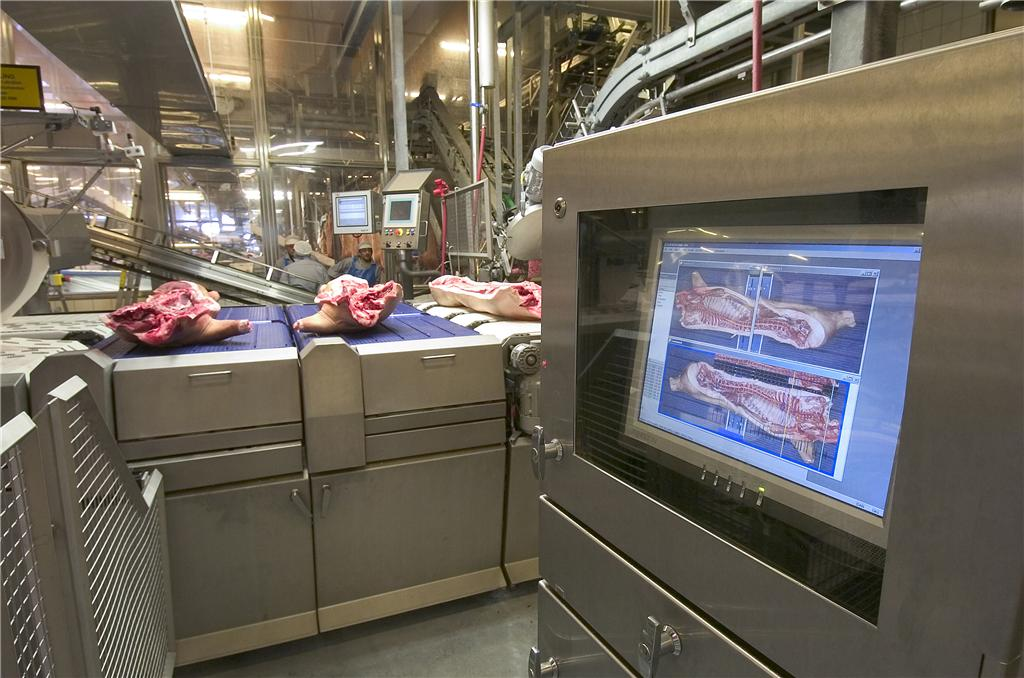
\includegraphics[scale=0.5]{images/209690-1}
	\caption{Billedet viser i forgrunden  et foto taget af tredeleren til brug for analyse. I baggrunden ses transportbåndet, hvor de halve  grise venter på på at blive udskåret af den automatisk tredeler.}
	\label{fig:pig}
\end{center}
\end{figure}


Slagteriet har placeret kameraet i starten af et transportbåndet mens udskæringsrobotten findes i den anden ende. Der kan være flere grise på transportbåndet på samme tid, og det fremfører grisene i et fast tempo. Dette giver et fast tidsrum fra grisen passerer kameraet til det passerer robotten. Vi har hermed et klassisk RTP system, hvor robotten skal foretage et valg under en hard deadline, da der skal foretages en udskæring.

Vi må først se på arbejdsgangen der er involveret i valget af model:
\begin{enumerate}
\tightlist
	\item Et billede bliver taget af grisen mens den passerer kameraet.
	\item Billedet konverteres til en 3D-model af grisen.
	\item 3D-modellen analyseres.
	\item Robotten udvælger hvor udskæringerne skal være på baggrund af analysen, ordren og kundens ønske.
	\item Robotten udskærer grisen.
\end{enumerate}

Man kan se at arbejdsgangen indeholder en  række klart afgrænsede arbejdsområder, som med fordel kan modelleres som selvstændige processer i \pycsp.  Vi har derfor valgt implementere følgende processer: Kamera, Billedekonvertering, 3D-analyse og en udvælgelse og udskæringsproces, hvilket leder til et procesnetværk som vist i \cref{fig:pig-network}.

\begin{figure}
 \begin{center}
  
\includegraphics[scale=1]{images/pig-network}
	\caption{Procesnetværk til udskæring af grise på et slagteri.}
	\label{fig:pig-network}
\end{center}
\end{figure}

\subsubsection*{Implementering}\label{sec:deadline-exampel-implementation}
Til at implementere eksemplet i \pycsp, kan vi oprette hvert gris som et objekt og tilknytte et tidspunkt dertil som vi kan bruge som en deadline. Med denne kan hver proces evaluere om grisen har overskredet sin deadline, og i det tilfælde fjerne griseobjektet, og stoppe den videre behandling af det. Da det er ikke angivet hvordan hele processen startes,  antager vi der findes en form for detektor foran kameraet, der opfanger når en gris passerer og som dermed starter processen. 

Når detektoren starter hele processen, opretter den et griseobjektet som den sender til kameraprocessen, samt sender en kopi direkte til udvælgelse og udskæringsprocessen. Dermed ved processen at der ankommer en gris som den skal udskære, og hvis den, inden deadline, får en analyse af grisen, kan den træffe et begrundet valg om hvordan udskæringen skal foretages. Hvis ikke denne analyse findes, bruges blot standardmodellen til at udskære grisen. \CRef{fig:pig-network2} viser det endelige  netværk, hvor detektoren er introduceret, og som sender data til hhv. kameraprocessen og til udvælgelse og udskæringsprocessen. 

\begin{figure}
 \begin{center}
  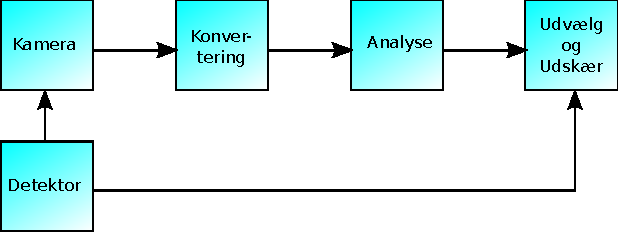
\includegraphics[scale=1]{images/pig-network2}
	\caption{Procesnetværk med detektor til initiering af hver gris.}
	\label{fig:pig-network2}
\end{center}
\end{figure}

Vi har holdt os tæt op af den virkelige verden, i designet af implementeringen, men da dette er et delvist tænkt eksempel har vi i  sagens natur ikke  adgang til slagteriet og deres maskiner, eller præcis data om grisene. Derfor må vi nødvendigvis simulere store dele af eksemplet. 

De enkelte processer foretager derfor ikke et konkret stykke arbejde, men har  tilknyttet et tal der repræsenterer det tidsrum, som vi forventer arbejdet i processen vil tage. Hver proces simulerer i stedet arbejdet, i et normalfordelt tidsrum omkring det tilknyttede tidsrum.

Detektoren starter processeringen af hver gris. Derfor står detektoren for oprettelsen af griseobjektet, hvori vi også  definerer om den har et ekstra sæt ribben. Denne oplysning bruges af de enkelte processer til at justere tidsrummet bearbejdningen af grisen tager. 

Et problem ved at implementere slagterieksemplet i \pycsp er  grænsefladen mellem verdenen hvor grisene kører på transportbåndet, og  koden. I \code{greenlets}-versionen.   er der kun  en proces  der er aktiv af gangen og denne kan være aktiv så længe den ønsker. Det er i eksemplet  krævet at  grisen bliver udskåret mens den er indenfor robottens rækkevidde, hvorfor det er uacceptabelt hvis ikke udvælg og udskæringsprocessen er aktiv i tidsrummet hvor grisen er inden for rækkevidde af robotten. 

For at  udvælg og udskæringsprocessen kan aktiveres skal konverterings- og analyseprocesserne frivilligt stoppe deres arbejde mens  udvælg og udskæringsprocessen foretager udskæringen.  Vi har dog ikke kendskab hvilket arbejde de to processer kommer til at foretage sig, og kan dermed heller ikke sige om det vil være muligt med regelmæssige mellemrum at afgive kontrollen. Hvis det er muligt for processerne at afgive kontrollen med jævne mellemrum, findes der heller ikke i \code{greenlets}-versionen mulighed for midlertidigt at lade andre processer  komme til hvis de ønsker det, og ellers fortsætter. Det bedste man vil kunne gøre, er at benytte en  \code{alternation} med en \code{timeout}. Dette vil dog samtidigt sænke ydelsen da  processen med alternation dermed er tvunget til at vente i minimum i denne timeout. 

Alternativt kan processerne deles op i to separate applikationer. En applikation skrevet i \pycsp der skal stå for konvertering og analyse mens en anden skal styre robotten. De to applikationer skal kunne kommunikere og  udveksle data, f.eks. igennem en database, harddisk eller anden delt datastruktur. Hvis analysen bliver færdig gemmes den i den delte datastruktur og applikationen der styrer robotten kan udnytte analysen. Hvis ikke den er klar bruges i stedet standardmodellen. Som beskrevet i \autoref{chap:csp} og som vi også kom ind på i implementeringen i \autoref{sec:des-examples}, strider en delt datastruktur dog mod ideerne i CSP, hvorfor det ikke er optimalt.

I stedet for at vælge \code{greenlets}-versionen kunne man i stedet vælge \code{process}-versionen. Hermed vil man kunne køre processer samtidigt, og udnyttet operativsystemet til at foretage preemptive afbrydelse af  processerne, således at alle samtidigt får en del CPU-tid. Dermed kan alle tre processer kører samtidigt og robotten kan foretage udskæringen. \code{Process}-versionen risikere dog at operativsystemet foretager en preemptiv processkift, mens udskæringsprocessen kører, således at konvertering og  analyseprocessen også kan arbejde. Potentielt vil dette kunne resultere i at grisen ikke bliver udskåret, selvom griseobjektet ankommer rettidigt til udvælg og udskæringsprocessen.

Med tanke på de ovenstående fordele og ulemper der findes ved hhv.  \code{greenlets}-versionen og \code{process}-versionen,  har vi valgt at implementere begge versioner for i evalueringen at sammenligne dem med RTP-versionen. Fra et praktisk synspunkt vil \code{greenlets}-versionen ikke være relevant, da denne har nogle flere ulemper end \code{process}-versionen. Men til at danne grundlaget for en sammenligning med RTP-versionen har den sin berettigelse.

I \code{greenlets}-versionen er ``Udvælgelse og udskæringsprocessen'' reduceret til en IO-proces der modtager grisene og gemmer dem så en anden applikation kan tilgå dem. Til dette har vi valgt at bruge en \code{dictonary} datastruktur til at gemme  hver gris under deres unikke id. Første gang processen modtager en gris gemmes den i datastrukturen, så i tilfælde af at analysen ikke bliver færdig vil den anden applikation som minimum vide der kommer en gris. Anden gang den samme gris modtages er det fra analyseprocessen, med det færdige resultat hvorfor  den gamle gris overskrives. Den anden applikation, kender derfor til alle grisene, uanset om analysen er blevet rettidigt færdig.

\code{Process}-versionen, er magen til \code{greenlets}-versionen, men den praktiske forskel at processerne kører som selvstændige python-processer og derfor har muligheden for parallel kørsel. 

\fxwarning{konsekvent brug af process- vs processes-versionen}

%\subsection{Eksempel 2 - Sensornetværk med høj/lav -prioritet}
%\inline{eks2: skal vise alternation, kan være en sensor som modtager måledata med lav prioritet og som skal sende måledata på opdordring med høj prioritet.}
